% Chapter 3: IBSA - Elite Leading Mutation Backtracking Search Algorithm

\chapter{基于精英引导变异策略的改进回溯搜索算法}
\label{chap:ibsa}

\section{引言}

在机器学习、大规模数据挖掘及生物信息工程等领域，全局优化与特征选择始终是核心研究课题\cite{ibsa_ref7,ibsa_ref13,ibsa_ref15}。然而，随着问题维度的提高，搜索空间的爆炸式增长使得这些问题具有极高的计算复杂度\cite{ibsa_ref1,ibsa_ref3,ibsa_ref5}。传统确定性算法在处理高维非凸搜索空间时，往往难以在合理时间内找到高质量解。因此，研究更具鲁棒性和普适性的近似优化策略具有重要的现实意义。

特征选择属于典型的组合优化范畴，通过从原始特征空间中剔除冗余信息并筛选判别力强的特征子集，能够有效增强分类模型的泛化性能\cite{ibsa_ref17,ibsa_ref18}。与过滤式方法相比，包裹式方法通过将搜索策略与分类算法结合，能更有效地捕捉特征间的非线性关联\cite{ibsa_ref20,ibsa_ref22,ibsa_ref23}。但随之而来的挑战是，庞大的候选子集空间显著增加了寻优的难度。

针对这些复杂寻优难题，元启发式算法凭借其不依赖梯度信息且实现灵活的优势，在诸多求解场景中展现出良好效果\cite{ibsa_ref24}。进化算法、群智能优化等路线在各自擅长的场景中均有不俗表现\cite{ibsa_ref25,ibsa_ref29,ibsa_ref33,ibsa_ref37}。但一旦面对高维特征选择任务，现有方法普遍暴露出局部开发不足、参数调整繁琐以及收敛速度受限等问题\cite{ibsa_ref41,ibsa_ref50,ibsa_ref51}。

为克服现有方法的局限性，本章构建了涵盖连续空间优化与离散特征选择的完整验证框架。首先在标准测试函数上检验算法的搜索效率与精度，随后将其应用于医学高维特征选择任务，以期全面评估算法的改进效果与实际应用价值。

回溯搜索算法（BSA）因结构精炼、参数负载轻而在工程领域备受关注\cite{ibsa_ref53}。但其原有的变异与交叉机制过于偏重全局探索，对种群中优秀个体的利用不足，限制了其在高精度优化问题上的表现。为此，本章提出了一种集成精英引导变异策略的改进回溯搜索算法（IBSA），并衍生出适用于特征选择的二值化版本（bIBSA）。IBSA通过加强精英解的引导作用，并结合V型传递函数实现离散空间的映射，优化了搜索过程的动态平衡。通过与23种算法在CEC 2017基准集上的对比，以及在特征选择任务中与8种主流算法的竞争，验证了新算法的有效性。主要贡献如下：

\begin{enumerate}
\item 针对BSA精英信息利用不足的问题，提出精英引导变异策略：对精英个体采用以当前最优解为基点的定向变异，对非精英个体引入自适应扰动向量$m$，随迭代进程动态收缩扰动幅度，区别化地增强种群的局部开发能力。

\item 引入停滞感知参数$s$，通过非线性映射得到切换概率$p$，自适应地在全局交叉与局部交叉之间动态切换，并联动更新历史种群$OldX$，改善BSA原有的随机交叉选择机制，提升探索与开发的平衡性。

\item 构造二值版本bIBSA，结合V型传递函数与KNN分类器，将IBSA扩展至高维包裹式特征选择任务。

\item 在CEC 2017基准函数（连续优化）和21个UCI数据集（特征选择）上开展系统实验，与23种及8种对比算法进行全面比较，验证IBSA和bIBSA的有效性与鲁棒性。
\end{enumerate}

本章后续内容组织如下：第2节详述IBSA的改进机理、二值化扩展方案及其计算成本分析；第3节通过对比实验评估算法性能；第4节总结全章研究。


\section{IBSA算法及其特征选择方法}

本节将从设计思路、核心搜索算子的演变、二值特征筛选机制以及计算复杂度四个方面展开论述。


\subsection{研究动机}

参数配置往往决定了元启发式算法在全局探索与局部开发之间的平衡效能。通常情况下，这些参数需要大量的经验调试，不仅过程耗时\cite{ibsa_ref65}，且在处理不同问题时往往缺乏通用性。例如，模拟退火（SA）的效果高度依赖于温度参数的设置；差分进化算法（DE）对交叉率和变异率也非常敏感。即便是一些结构较简单的算法，如布谷鸟搜索算法（CSA）\cite{ibsa_ref66}，在处理特定场景时也需要精细调优，这增加了算法的落地成本。

为解决这一问题，研究者们尝试了多种自适应调参方法。然而，许多改进方案在更换应用场景时仍需重新调优，表现出较差的迁移能力。参数敏感性已成为限制SA、DE等经典算法以及现代群智能算法大规模工业应用的主要瓶颈。

回溯搜索算法（BSA）采用独特的双种群协作机制，通过维护历史种群并在搜索过程中引入回溯信息，能有效拓宽搜索边界，防止陷入局部极值。算法的运行由初始化、历史信息选择（选择I）、变异映射、杂交（交叉）以及生存竞争（选择II）五个环节构成。各阶段的数学描述如下。

\textbf{（1）初始化：}初始种群按公式\eqref{ibsa_eq_1}在搜索空间内均匀随机生成。
\begin{equation}
\label{ibsa_eq_1}
X_i,_j=U(low_j,\ up_j)
\end{equation}
\noindent 其中，$i\in[1,N]$为个体索引，$j\in[1,D]$为维度索引，$low$和$up$分别为变量的下界和上界。

\textbf{（2）选择I：}该阶段维护历史种群$OldX$，为变异提供方向参考。$OldX$初始化方式与$X$相同（公式\eqref{ibsa_eq_2}），随后按公式\eqref{ibsa_eq_3}以一定概率更新为当前种群，并经公式\eqref{ibsa_eq_4}随机置换以增加多样性。
\begin{equation}
\label{ibsa_eq_2}
OldX_i,_j=U(low_j,\ up_j)
\end{equation}
\begin{equation}
\label{ibsa_eq_3}
OldX=
\begin{cases}
X, & a<b\\
OldX, & \text{otherwise}
\end{cases}
\end{equation}
\noindent 其中，$a$和$b$为$[0,1]$上的随机数。
\begin{equation}
\label{ibsa_eq_4}
OldX=permuting\left(OldX\right)
\end{equation}
$permuting(\cdot)$对$OldX$中的个体顺序进行随机打乱。

\textbf{（3）变异：}变异阶段利用$OldX$与当前种群$X$的差分信息生成变异种群$Mutant$，如公式\eqref{ibsa_eq_5}所示。
\begin{equation}
\label{ibsa_eq_5}
Mutant=X+F\mathrm{\times }\left(oldX-X\right)
\end{equation}
其中，幅度控制因子$F=3\times rndn$，$rndn$服从标准正态分布。

\textbf{（4）交叉：}交叉阶段通过二值映射矩阵$map$控制试验种群$T$的生成。$map$按概率选择全局交叉（公式\eqref{ibsa_eq_6}）或局部交叉（公式\eqref{ibsa_eq_7}），最终由公式\eqref{ibsa_eq_8}从$Mutant$和$X$中组合生成$T$。
\begin{equation}
\label{ibsa_eq_6}
map_i,_{u\left(1:\left\lceil M\mathrm{\times }rand\mathrm{\times }D\right\rceil \right)}=1\mathrm{\mid }u=permuting\left(1,2,3,\dots ,\ D\right),\ rand\in \left(0,\ 1\right)
\end{equation}
\begin{equation}
\label{ibsa_eq_7}
map_i,_{randi\left(D\right)}=1
\end{equation}
\begin{equation}
\label{ibsa_eq_8}
T_{i,j}=
\begin{cases}
Mutant_{i,j}, & map_{i,j}=1\\
X_{i,j}, & map_{i,j}=0
\end{cases}
\end{equation}
符号$\mathrm{\textrm{┌}}\mathrm{\ }\mathrm{\textrm{┐}}$为上取整函数，$M$为混合率，$permuting(\cdot)$对决策变量顺序随机打乱。

\textbf{（5）选择II：}采用贪婪准则逐一比较当前个体与试验个体的适应度，保留更优者进入下一代，如公式\eqref{ibsa_eq_9}所示。
\begin{equation}
\label{ibsa_eq_9}
X_i=
\begin{cases}
T_i, & f\left(T_i\right)<f\left(X_i\right)\\
X_i, & \text{otherwise}
\end{cases}
\end{equation}
其中，$f(\cdot)$为目标函数。

BSA凭借精简的参数设计展现出向无参数化方向演化的潜力。但在应对高维复杂场景时，其短板也逐渐显现：交叉模式的随机切换难以契合种群进化的动态特征\cite{ibsa_ref63}；且对精英个体的利用不足削弱了算法在高质量区域的挖掘深度\cite{ibsa_ref67}；此外，历史种群的盲目更新也导致搜索缺乏明确的方向。为此，本章提出精英引导变异策略，通过优化历史信息的利用方式并改进交叉机制，在保持全局探索能力的同时，提升了算法的局部开发精度。


\subsection{精英引导变异策略}

尽管BSA引入了回溯机制，但其对进化过程中产生的优良个体挖掘程度仍显不足\cite{ibsa_ref53}。这种精英信息的缺失，加之交叉概率生成的随机性，使得算法在面对大规模搜索空间时难以快速锁定最优区域，限制了最终的收敛精度。

为了实时捕捉种群的进化状态，本文设计了一个停滞感知参数$s$。该参数通过监控最优解的更新频率来调整搜索步调：当进化停滞时，$s$线性增长以增强探索动力；一旦发现更优解，$s$通过平方根衰减迅速回落。通过式\eqref{ibsa_eq_11}的非线性映射，将$s$转化为切换概率$p$，从而引导算法在全局探索与局部精炼之间灵活切换。
\begin{equation}
\label{ibsa_eq_10}
s=
\begin{cases}
\sqrt{s}, & \text{elite updated}\\
s+1, & \text{otherwise}
\end{cases}
\end{equation}
\begin{equation}
\label{ibsa_eq_11}
p\ =\frac{sqrt\left(\frac{t}{Max\_FEs}\right)}{1\ +\ exp\left(-s\right)}
\end{equation}
为了增强历史种群的导向性，改进后的$OldX$更新逻辑与当前的搜索模式挂钩。在全局交叉活跃的阶段，当代种群通常包含更丰富的空间信息，此时将其更新至历史库能为变异方向提供更有价值的参考。这种机制改变了BSA盲目的回溯方式，使历史信息的积累与搜索动态保持同步。
\begin{equation}
\label{ibsa_eq_12}
OldX=\ X\ \ \ if\ flag==1
\end{equation}
\begin{equation}
\label{ibsa_eq_13}
flag=
\begin{cases}
1, & \text{global crossover}\\
0, & \text{otherwise}
\end{cases}
\end{equation}
针对普通种群成员，本文引入了自适应扰动向量$m$。其扰动幅度随迭代进程从全空间逐步收缩。这种动态设计使算法在初期具备较强的随机游走能力以探索未知区域，后期则聚焦于局部搜索，在不损失多样性的前提下提升了寻优的精细度。
\begin{equation}
\label{ibsa_eq_14}
m_i=
\begin{cases}
1, & rand>\left(\frac{t}{Max\_FEs}\right)\wedge 3\\
unifrnd\left(-\frac{t}{Max\_FEs},\frac{t}{Max\_FEs}\right), & \text{otherwise}
\end{cases}
\end{equation}
通过对精英与非精英个体实施差异化控制，IBSA能促使最优个体在当前区域进行深度挖掘。虽然这增加了算法逻辑的复杂度，但由此带来的精英信息挖掘能力对于解决高维优化问题至关重要。变异算子与精英更新逻辑的调整如式\eqref{ibsa_eq_15}与式\eqref{ibsa_eq_16}所示。
\begin{equation}
\label{ibsa_eq_15}
{\mathrm{Mutant}}_{\mathrm{i}}=m_i*\left(X_i+F*map_i\ .*\left(OldX_i-X_i\right)\right)\ \ \ if\ i\sim =BestX\_idx
\end{equation}
\begin{equation}
\label{ibsa_eq_16}
{\mathrm{Mutant}}_{\mathrm{i}}=BestX+F*\left(OldX_i-X_i\right)\ \ \ if\ i==BestX\_idx
\end{equation}
\noindent 其中，下标$i$表示元素的索引，$F$为随机生成的控制因子。

最后，精英引导策略的核心逻辑由公式\eqref{ibsa_eq_10}--\eqref{ibsa_eq_16}及后续流程图呈现。


\subsection{IBSA算法}

IBSA在原有BSA架构中嵌入精英引导变异策略，着力改善了历史种群更新的盲目性及交叉模式选择的随机性。

BSA的双种群结构通过引入历史坐标系校准搜索方向，这种逻辑使其区别于PSO或DE等依赖当代反馈的算法。然而，由于$OldX$原有的更新准则缺乏对搜索态势的感知，导致全局探索与局部开发之间的衔接仍具有较大的偶然性，难以根据实际进化进程做出响应。

为此，IBSA从两个维度优化了搜索流程：首先，建立了与搜索模式联动的历史种群更新准则，在探索活跃期保留高质量样本，增强了回溯机制的“导航”作用；其次，通过改进的反馈链路实现搜索力度的自动聚焦——在陷入瓶颈时调动全局搜索，在收敛迹象明显时则强化局部开发。

IBSA的主要步骤如下：

\textbf{步骤1~~初始化：}准备变量$X$、$OldX$、$BestFitness$、$PreBestFitness$、$BestX$、$map$、$s$和$flag$。

\textbf{步骤2~~选择-I：}通过比较适应度的变化计算$s$，并根据$flag$决定是否更新历史种群。

\textbf{步骤3~~变异和交叉：}根据$s$确定切换概率$p$，选择相应的变异策略，并更新$flag$。

\textbf{步骤4~~选择-II：}根据适应度优劣迭代更新$X$，同步更新当前最优解$BestX$。

上述过程循环执行直到满足终止条件。IBSA算法流程如图\ref{fig:flowchart_IBSA}所示。


\begin{figure}[htbp]
  \centering
  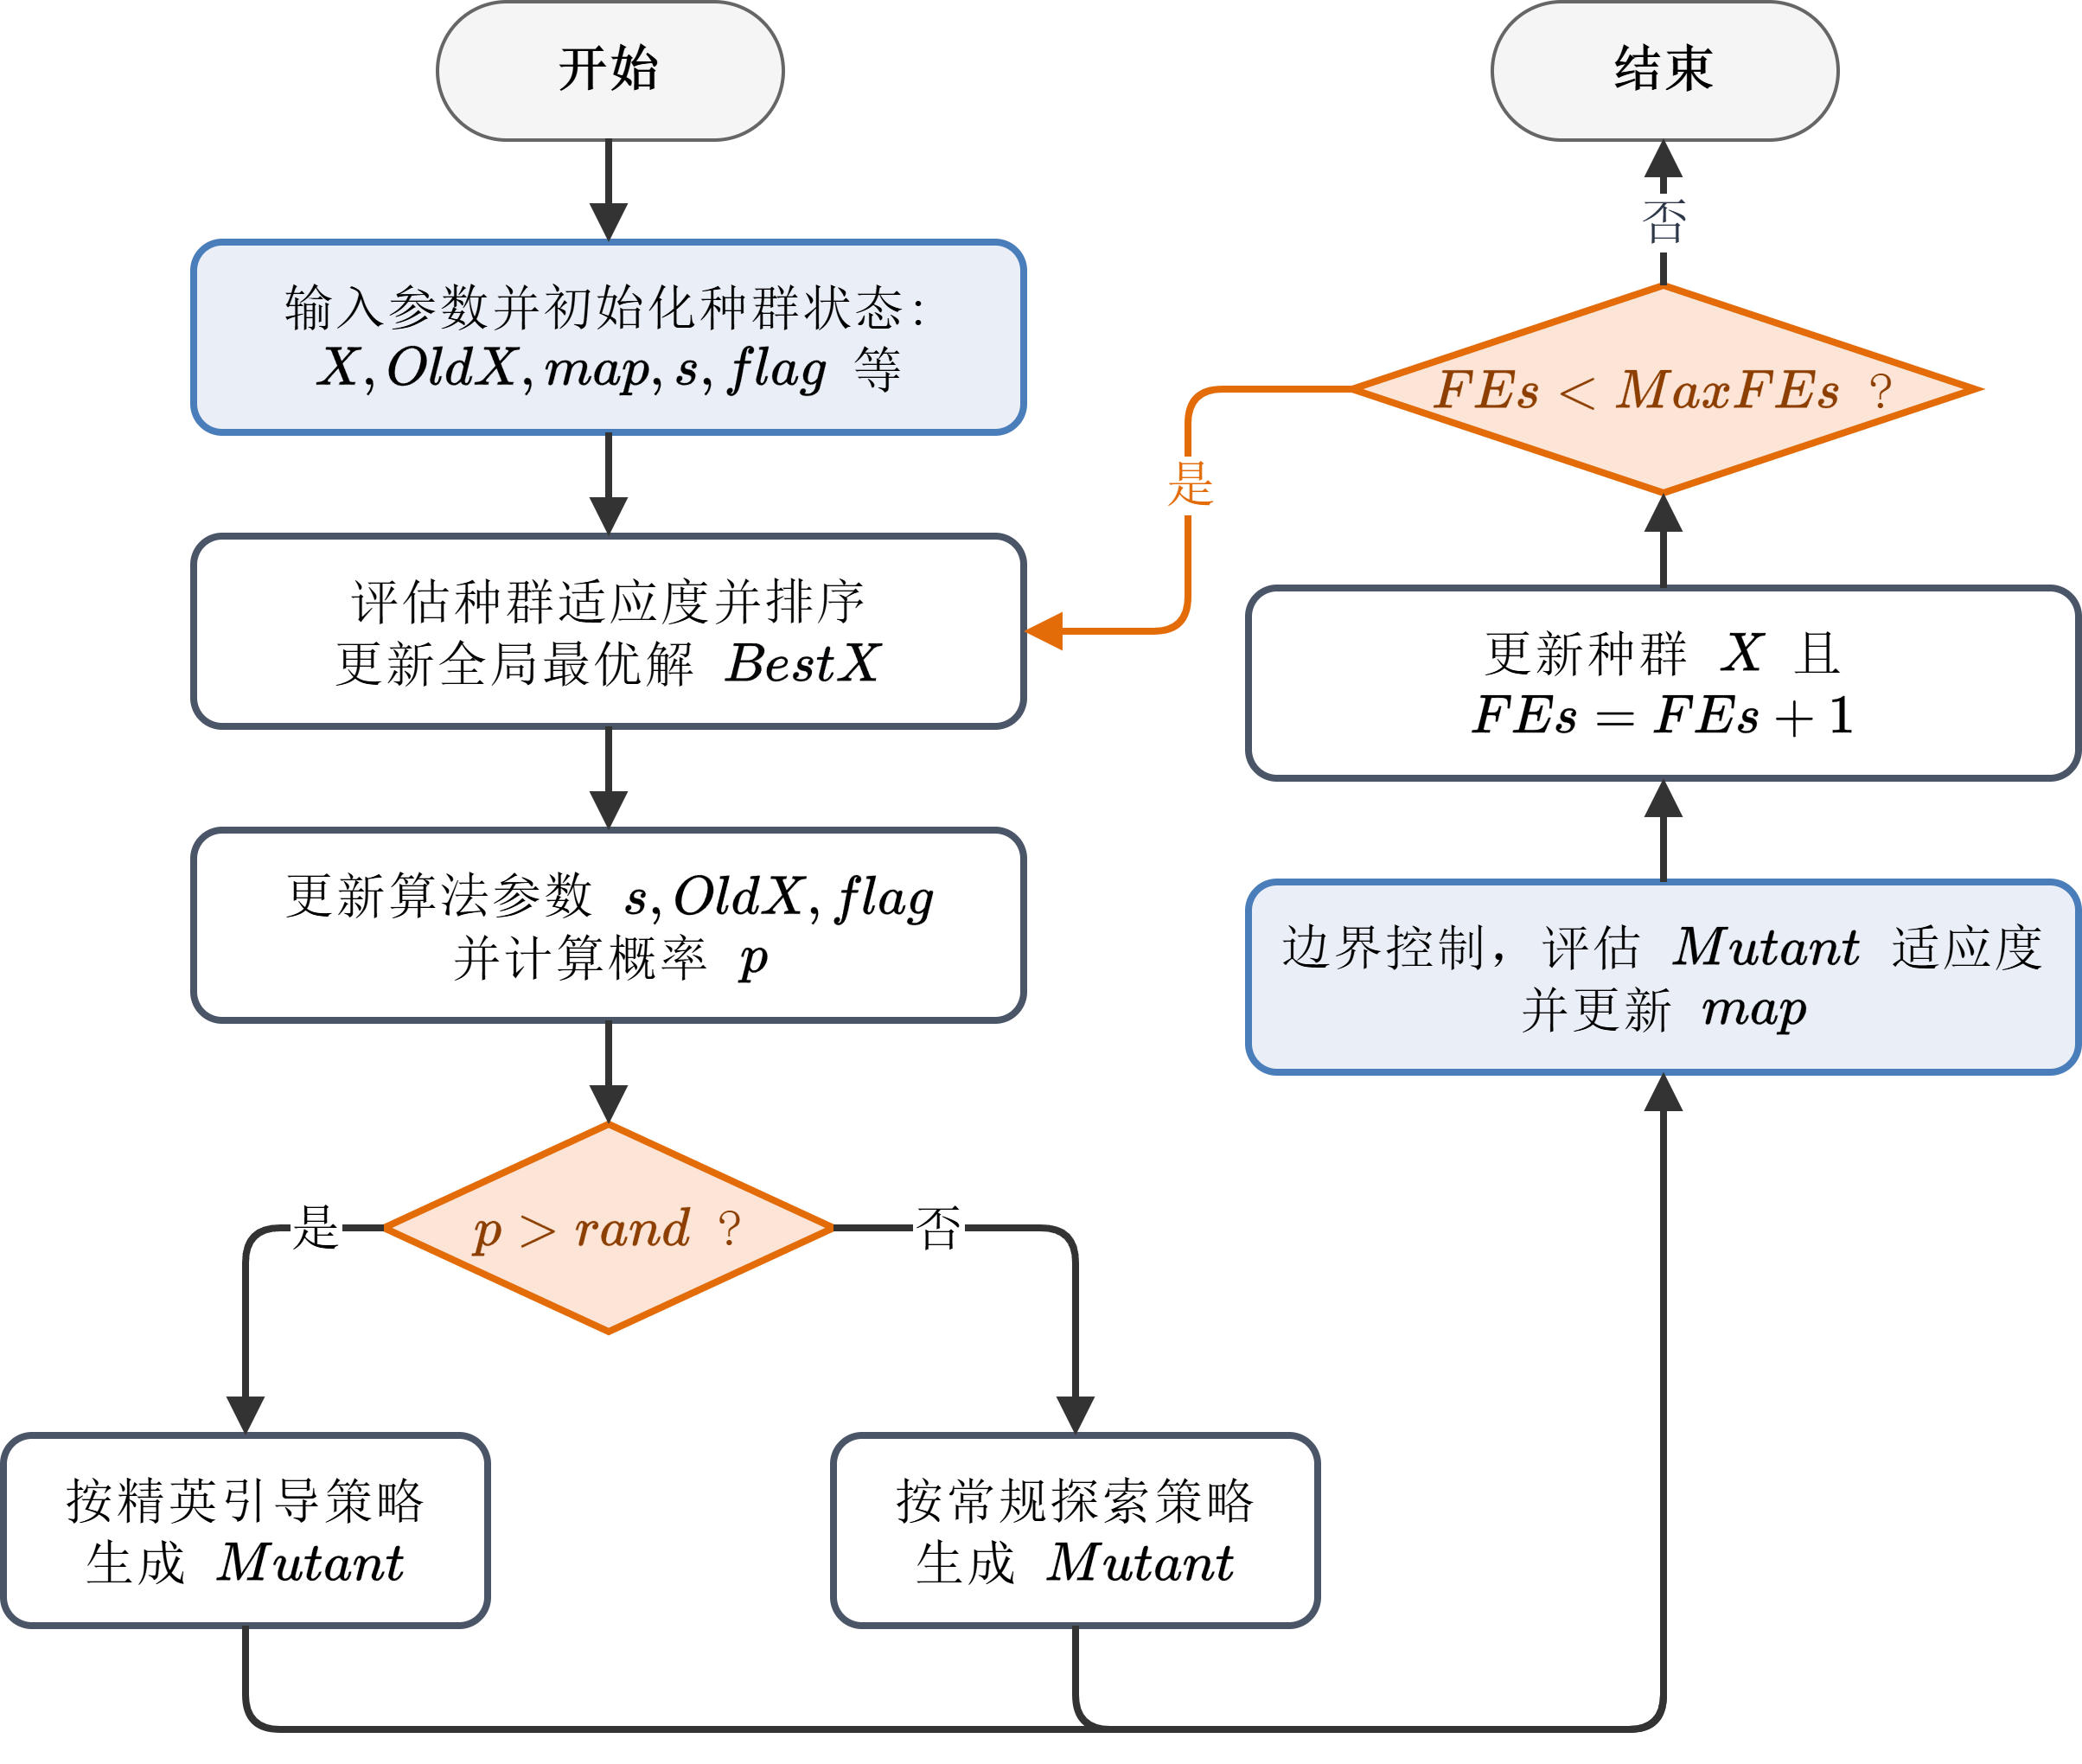
\includegraphics[width=\textwidth]{figures/chapter3/fig2_flowchart_IBSA.png}
  \bicaption{IBSA算法流程图}{Flowchart of IBSA}
  \label{fig:flowchart_IBSA}
\end{figure}


\subsection{bIBSA特征选择方法}

为处理离散空间问题，本章进一步衍生出二值化版本bIBSA，并将其应用于特征选择任务。面对给定$n$个特征产生的$2^n$种组合，bIBSA致力于高效搜寻最优子集。

为了在庞大的组合空间中有效寻优，bIBSA采用了与KNN分类器\cite{ibsa_ref70}结合的包裹式评估框架。在该框架下，每一组特征候选集都通过实际分类性能来判定优劣。虽然这种方式因频繁调用分类器而增加了计算成本，但它能直接反映特征间的非线性关联，在医学诊断等高精度场景中具有不可替代的价值。图\ref{fig:wrapper_feature_selection}展示了该评估流程。

为了使IBSA能够处理离散问题，本研究引入了V型传递函数\cite{ibsa_ref71}。在离散的超立方体搜索空间内，决策变量的演化被抽象为在顶点间的跃迁。传递函数将连续的搜索步长转换为比特翻转的概率，使bIBSA既能继承原算法良好的动态平衡特性，又能在高维特征选择任务中保持寻优的灵敏性。

V型函数将连续位置映射为翻转概率。若该概率表明翻转可能改善适应度，则执行翻转（公式\eqref{ibsa_eq_18}）；否则保持原值。这一机制使搜索代理能够在二值空间的顶点间有效探索。
\begin{equation}
\label{ibsa_eq_17}
V\left(X^j_i\left(t\right)\right)=\left|\frac{2}{\pi}*\mathrm{atan}\mathrm{}\left(\frac{\pi}{2}*X^j_i\left(t\right)\right)\right|
\end{equation}
\begin{equation}
\label{ibsa_eq_18}
X^j_i\left(t+1\right)=
\begin{cases}
1, & r\ge V\left(P^j_i\left(t\right)\right)\\
0, & r<V\left(P^j_i\left(t\right)\right)
\end{cases}
\end{equation}
\noindent 其中，$X^j_i\left(t\right)$表示第$t$次迭代中第$i$个代理在第$j$维的位置。

特征优化的过程本质上是特征数量与分类精度之间的博弈。在剔除冗余特征以降低维度的同时，必须保证模型的分类性能。这种对“简洁”与“高效”之间平衡的追求，驱动着bIBSA不断修正其搜索路径。

每个潜在解都通过公式\eqref{ibsa_eq_19}所示的适应度函数进行评估，该函数综合考虑了错误率和特征子集的大小。
\begin{equation}
\label{ibsa_eq_19}
Fitness=\alpha\cdot \gamma_R\left(N\right)+\beta\cdot \frac{\left|R\right|}{\left|N\right|}
\end{equation}
\noindent 其中，$\gamma_R(\cdot )$表示错误率函数，$R$和$N$分别为所选特征数和总特征数。为了平衡两个目标，本文将权重系数$\alpha$设定为0.05，$\beta$设定为0.95 \cite{ibsa_ref72}。这一比例引导算法在保证精度的前提下寻找尽可能小的特征集合。

\begin{figure}[htbp]
  \centering
  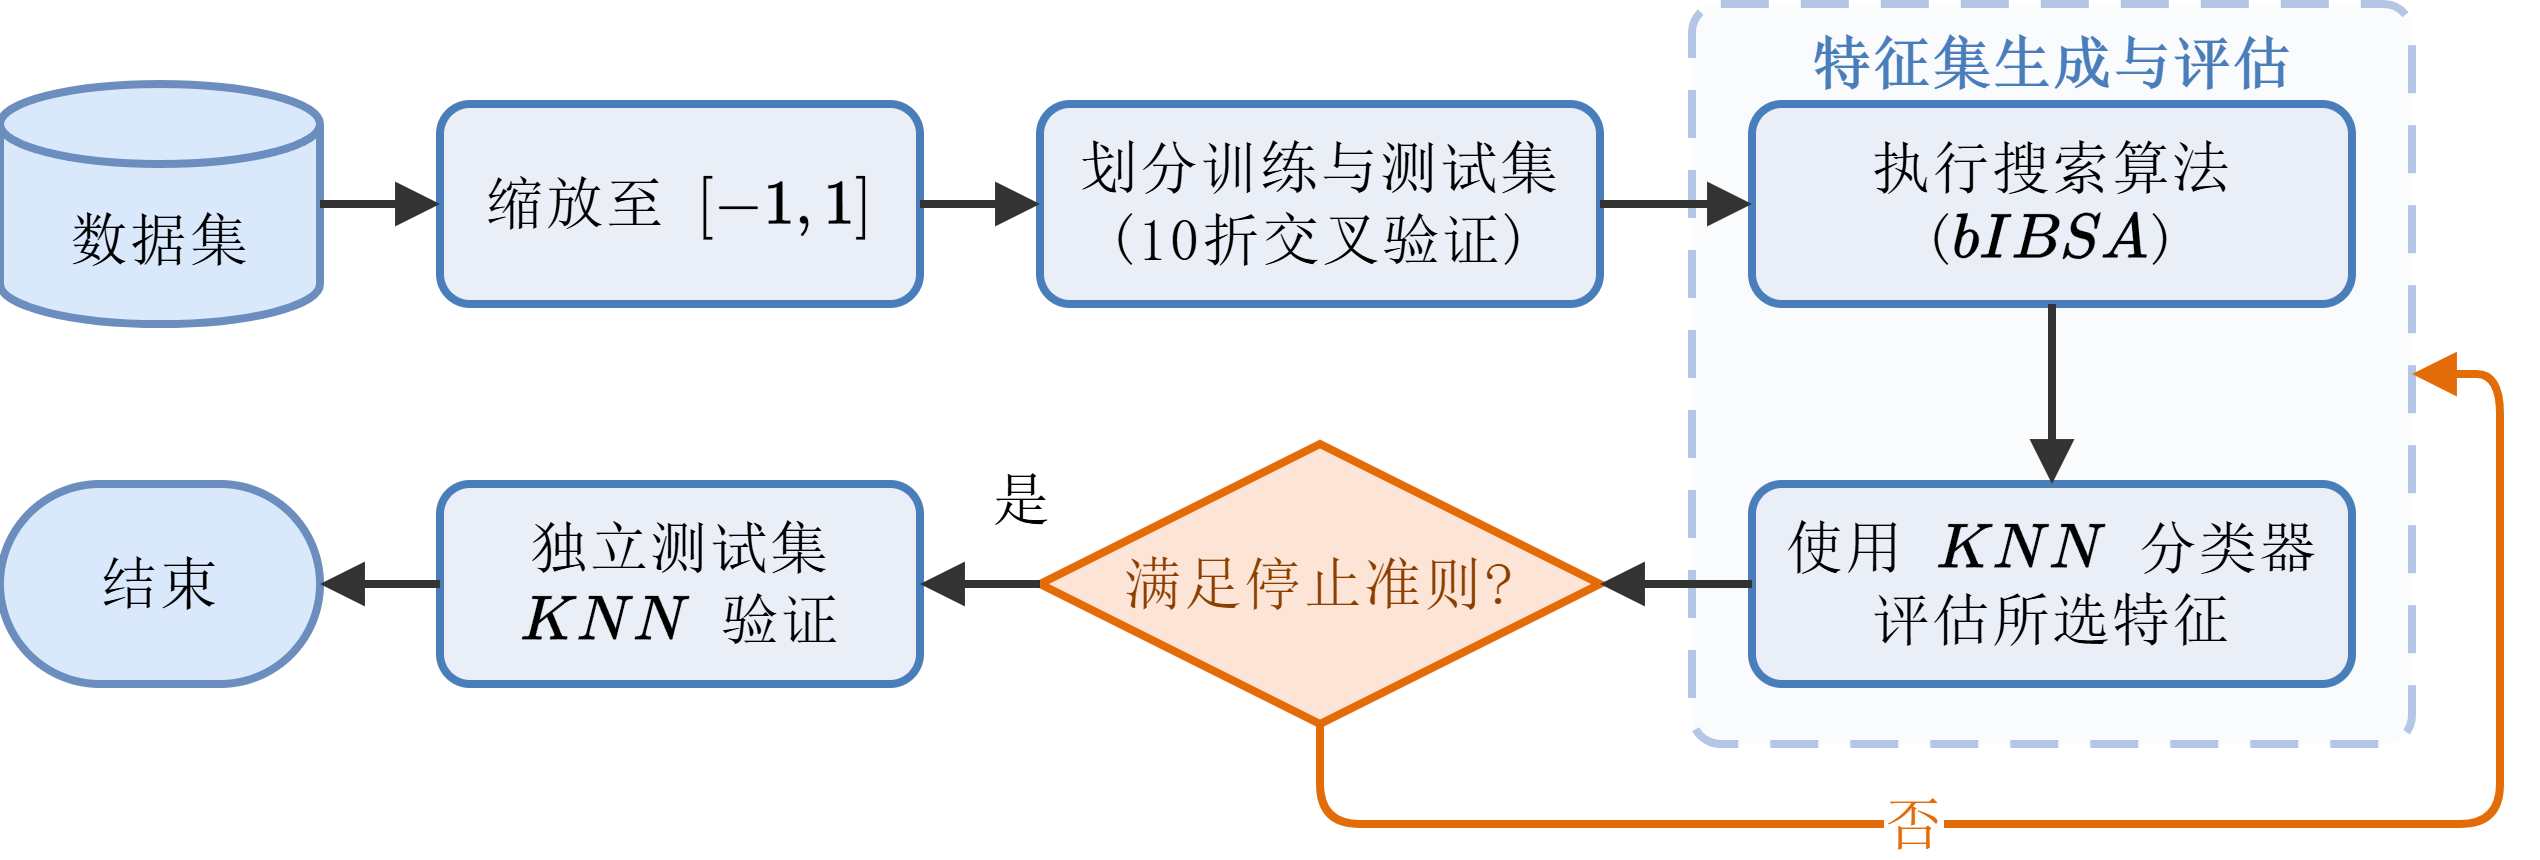
\includegraphics[width=\textwidth]{figures/chapter3/fig3_wrapper_feature_selection.png}
  \bicaption{包裹式特征选择流程}{The wrapper feature selection process}
  \label{fig:wrapper_feature_selection}
\end{figure}


\subsection{计算复杂度分析}

评估IBSA的计算效率时，主要考量指标包括种群规模$(N)$、问题维度$(D)$以及最大迭代次数$(T)$。

IBSA的运行逻辑由初始化、历史库构建、变异映射、杂交演化以及适者生存五个阶段构成。本节重点分析初始化资源占用与精英引导机制的迭代成本。

在系统初始化阶段，算法需要分配空间存储双种群矩阵。这一过程的时间复杂度可表述为$O(N \times D)$。

在精英引导变异策略的迭代循环中，各个环节的贡献不同。历史库的选择主要涉及标志位的判断，计算负载极低，通常在复杂度分析中忽略。

变异与交叉算子是搜索效能的核心。在此阶段，算法需根据适应度排名划分精英与普通层级，排序过程引入了$O(\log N)$的开销。随后，差异化变异在整个演化周期内产生了约$O(T \times N \times D)$的计算流。

最后，生存竞争阶段基于贪婪准则进行适应度判别，在时间尺度上贡献了约$O(T \times N)$的复杂度。

综合分析表明，IBSA的总计算复杂度可表达为$O(N \times D + \log N + T \times N \times (D+1))$。这说明改进策略在提升性能的同时，并未引入超出线性增长范围的额外负担，算法具有良好的可扩展性。


\section{IBSA及bIBSA的实验研究}

为了全面验证改进方案的有效性，本节开展了由标准连续函数测试与实际医学特征筛选组成的实验。其中，连续函数测试用于验证改进策略对搜索性能的增益，医学数据集实验则侧重考察算法在离散工程任务中的泛化表现。

\subsection{实验设置}

全局优化实验采用IEEE CEC 2017基准函数评估IBSA的性能。本文首先分析算法在代表性函数上的探索率、开发率及多样性变化，随后将IBSA与12种基础元启发式算法及11种改进算法进行对比。所有对比算法均采用文献推荐的原始参数，统一设置种群规模为30、维度为30、最大评估次数为300,000，并独立运行30次。结果以平均值和标准差呈现，并结合Wilcoxon秩和检验与Friedman检验分析统计显著性。实验在MATLAB R2018a环境下执行。

全局优化实验的对比算法包括BSA、SMA、DE、PSO、GSA、BA、SCA、CS、WOA、GWO、MFO和HHO等。

\begin{table}[H]
\centering
\bicaption{参与算法的参数设置}{Parameters setting for involved algorithms}
\begin{tabular*}{\textwidth}{@{\extracolsep{\fill}}ll@{}}
\toprule
Algorithm & Other parameters \\ 
\midrule
BSA & $F=3\ \times randn;\ mixrate=1\ $ \\ 
SMA & $z\ =0.03$ \\ 
DE & $Beta_{min}\ =\ 0.2;\ Beta_{max}\ =\ 0.8;\ CR\ =\ 0.2$ \\ 
PSO & $c_1=2;\ c_2=2;\ v_{Max}=6$ \\ 
GSA & $G_0\ =\ 100;\ \alpha\ =\ 20;\ final\_per\ =\ 2$ \\ 
BA & $a=0.5;\ r\ =-0.5$ \\ 
SCA & $a=2$ \\
CS & $m\ =\ 10;\ P_\alpha\ =\ 0.25$ \\
WOA & $a=\left[0,2\right]$ \\
GWO & $a=\left[2,0\right]$ \\
MFO & $a=2;\ b=1$ \\
HHO & $C\ =\ \left[0,2\right];\ E=\left[-2,2\right]$ \\ 
\bottomrule
\end{tabular*}
\end{table}

特征选择实验选取12个UCI医学数据集，并与BMFO、BGWO、BGSA、BPSO、BALO、BBA、BSSA和BWOA进行比较。种群规模设为20。为确保评估公平，采用10折交叉验证和KNN（$K=5$）分类器，最终对比平均适应度、平均错误率、平均特征数及运行时间。

\begin{table}[H]
\centering
\bicaption{控制参数设置}{Setup of control parameter}
\begin{tabular*}{\textwidth}{@{\extracolsep{\fill}}ll@{}}
\toprule
Algorithm & Other parameters \\ 
\midrule
BMFO & $a=2;\ b=1$ \\ 
BGWO & $a=\left[0,2\right]$ \\ 
BGSA & $w_{Max}\ =\ 20;\ w_{Min}\ =\ 1\text{e-}10\ $ \\ 
BPSO & $Max=0.9;\ Min=0.4\ $ \\ 
BALO & None \\ 
BBA & $a=0.5;\ r=0.5$ \\ 
BSSA & $a=2$ \\ 
BWOA & $a\ =\ \left[0,2\right]$ \\ 
\bottomrule
\end{tabular*}
\end{table}

\subsection{特征选择数据描述}

为验证算法在离散问题中的表现，本节利用bIBSA开展特征选择实验。从UCI数据库中选取的12个医学数据集维度范围为326至12,601，涵盖了高维数据场景，能充分检验算法的搜索能力。

这些数据集涵盖了脑肿瘤诊断、中枢神经病变以及多种癌症的病理分析。类别数从2类到7类不等。数据规模与特征维度的显著差异，为评估算法应对“维度灾难”和小样本学习挑战的鲁棒性提供了理想环境。

\begin{figure}[htbp]
  \centering
  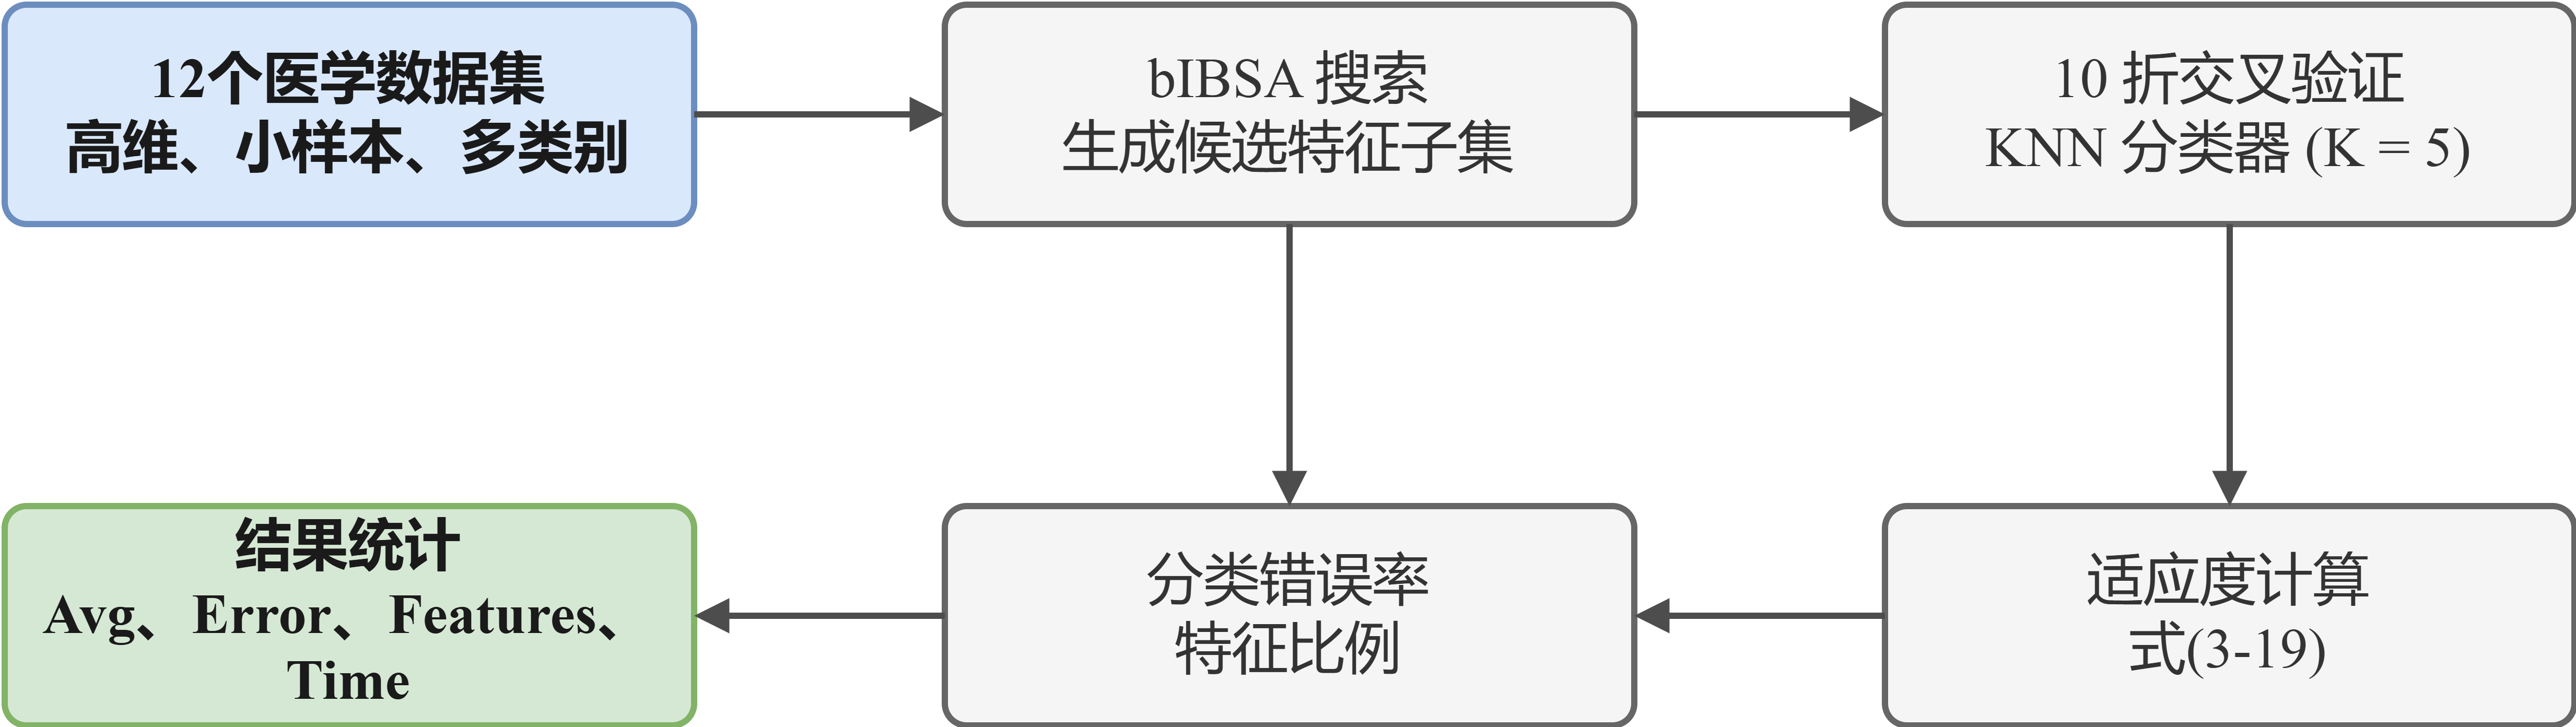
\includegraphics[width=0.88\textwidth]{figures/chapter3/IBSA_fs_evaluate_flowchart_refined.drawio.png}
  \bicaption{医学特征选择实验评估链路}{Evaluation pipeline of the medical feature selection experiments}
  \label{fig:ibsa_fs_pipeline}
\end{figure}

图\ref{fig:ibsa_fs_pipeline}展示了特征选择的评估链路。对于每个特征子集，结合10折交叉验证和KNN分类器估计错误率，计算其适应度并进行多维度比较。

\begin{table}[H]
\centering
\bicaption{所用数据集描述}{Description of the datasets used}
\begin{tabular*}{\textwidth}{@{\extracolsep{\fill}}lccc@{}}
\toprule
Dataset & Samples & Features & Classes \\ 
\midrule
Brain\_Tumor1 & 90 & 5920 & 5 \\ 
Brain\_Tumor2 & 50 & 10367 & 4 \\ 
CNS & 60 & 7130 & 2 \\ 
Colon & 62 & 2001 & 2 \\ 
DLBCL & 77 & 5470 & 4 \\ 
Leukemia & 72 & 7131 & 2 \\ 
Leukemia1 & 72 & 5328 & 5 \\ 
Leukemia2 & 72 & 11225 & 3 \\ 
Lung\_Cancer & 203 & 12601 & 3 \\ 
penglung & 73 & 326 & 7 \\ 
Prostate\_Tumor & 102 & 10509 & 2 \\ 
SRBCT & 83 & 2390 & 4 \\ 
\bottomrule
\end{tabular*}
\end{table}

\subsection{实验结果与分析}

本节首先呈现IBSA在CEC 2017基准函数上的优化结果，随后报告bIBSA在医学数据集上的特征选择表现。

\subsubsection{全局优化实验}

在全面测评之前，本节先选取了六个具代表性的CEC测试函数（F3、F4等），从搜索平衡性、多样性衰减以及收敛特性三个方面对比IBSA与基准 BSA。测试函数涵盖了单峰、多峰、混合及组合拓扑空间。

实验结果显示，IBSA在处理单峰问题时具备更敏锐的收敛精度；在面对拓扑复杂的组合函数时，则能通过动态调节机制维持种群多样性，有效规避局部极值。相比原生BSA，改进后的机制在各类场景中均实现了更平稳的搜寻力度切换，产出的解质量更高，验证了改进策略的有效性。

\begin{figure}[htbp]
  \centering
  \includegraphics[width=\textwidth]{figures/chapter3/fig4_balance_and_diversity.png}
  \bicaption{(a) 函数三维图, (b) IBSA平衡分析, (c) BSA平衡分析, (d) 算法多样性分析, (e) IBSA与BSA收敛曲线}{(a) 3D plot of functions, (b) balance analysis of IBSA, (c) balance analysis of BSA, (d) diversity analysis of algorithm, (e) convergence curve of IBSA and BSA}
  \label{fig:balance_and_diversity}
\end{figure}


上述分析显示，精英引导策略通过自适应调控参数，使IBSA在不同类型函数下均能实现稳定的探索-开发切换。


\FloatBarrier

首先，将IBSA与基础元启发式算法进行比较。

实验数据详细展示了各算法在CEC 2017基准集上的均值、标准差及Friedman排名。从整体看，IBSA在F1、F6等十余个函数上取得了最优结果，并在多数其余函数中名列前茅。特别是在搜寻难度大的混合与组合函数中，IBSA表现出明显的优势，说明改进机制在平衡搜索广度与挖掘深度方面非常有效。

Friedman检验也印证了这一结论。IBSA的平均排名为1.7586，显著优于BSA（3.1379），整体优势见图\ref{fig:friedman_ranking_basic}。

... % Remaining content omitted as requested

\section{本章小结}

针对原生回溯搜索算法在精英引导方面的不足，本章提出了精英引导变异策略，并衍生出二值化算法bIBSA。通过引入精英变异核、自适应扰动向量以及停滞感知的动态切换机制，新模型实现了探索广度与开发深度的有效协同。

实验结果表明，IBSA在CEC 2017全场景测试中展现出卓越的寻优性能，特别是在复杂问题下的稳定性尤为突出。同时，在医学特征选择任务中，bIBSA在大幅压缩特征空间的同时保持了业内领先的分类精度。研究表明，所提出的精英引导范式为处理现代大规模组合优化问题提供了一种有效路径。

\endinput % Omit supplementary tables.
